197. \begin{figure}[ht!]
\center{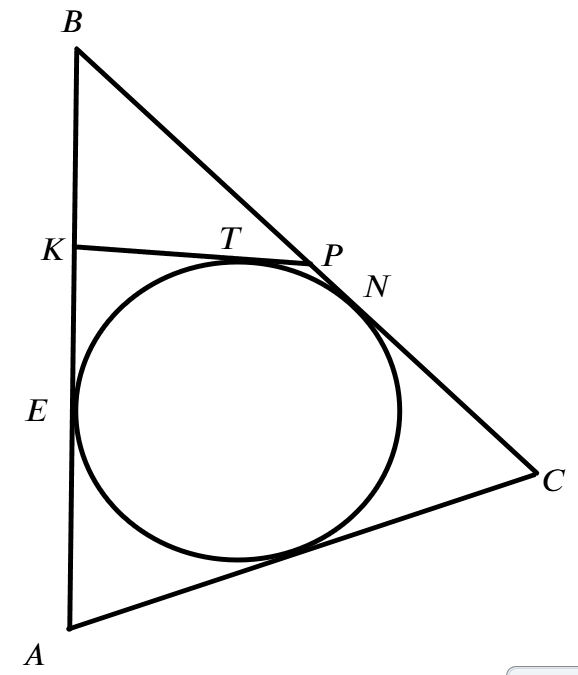
\includegraphics[scale=0.35]{g9-197.png}}
\end{figure}\\
Так как отрезки касательных, проведённых из одной точки, равны, имеем равенства $KE=KT,$ $PN=PT,\ BE=BN,$ откуда $P_{\Delta BKP}=BK+BP+KP=BK+BP+KT+PT=
BK+BP+KE+PN=BE+BN=2BE=2\cdot7=14.$\newpage\noindent
